%----------------------------------------------------------------------------------------
% SECTION 2
%----------------------------------------------------------------------------------------
\section{Elemental quantification of single layer systems}

% model performance
The model performance for the quantitative assessment of chemical composition is shown in Table \ref{tab:acc_quant}. The mean squared errors were computed for the multi dataset for each model.
% experimental data (AG_AG etc.)
From all experimental data, $\nmultispectra$ elemental spectra were used for the quantitative prediction. 

\begin{table}[H]
    \centering
    \begin{tabular}{c|c|c|c|c|c}
        &    & No.  & Training & Validation*  & Test*    \\
         Dataset   & Model&Parameters &                           dataset & dataset & dataset         \\
        \hline
        multi  & CNN     &   9.1 M        &     35.5       &   25.95                 &  1.92      \\
               & CNN-DCT &  35.3 M        &    13.61          &    14.16            &   \textbf{3.83}   \\
               & CBAM    & 28.2 M         &    23.32         &    14.94             &  2.68   \\ % CBAM_512_3_ES_MAE_4
               & ViT     &   35.3 M     &    33.81       &      34.86    &   2.68        \\
    \end{tabular}
    \caption{Number of parameters and threshold accuracy of the models}
    \label{tab:acc_quant}
\end{table}

As the threshold accuracy represents the percentage of elements with >10\% proportional content correctly quantified within a $\pm$10\% relative margin, it can be well compared to an experienced researchers result. With a maximum threshold accuracy of 3.83\% however, we are far off a good result for our best model. The full prediction mapped as heatmap is shown in Figure \ref{fig:multi_best_model}. It is interesting that the model with the best performance on the dataset has the least performance on the training and validation datasets. This could be due to the model being more robust, however as it contains 35.3 M parameters to train, we would expect it to possibly overfit the data. Thus, the most probable explanation is that our training dataset is not sufficient both in terms of number and resemblance to experimental data. For our best model, the mean absolute error per element is plotted in Figure \ref{fig:boxplot}.

\begin{figure}
    \centerline{
    \centering
    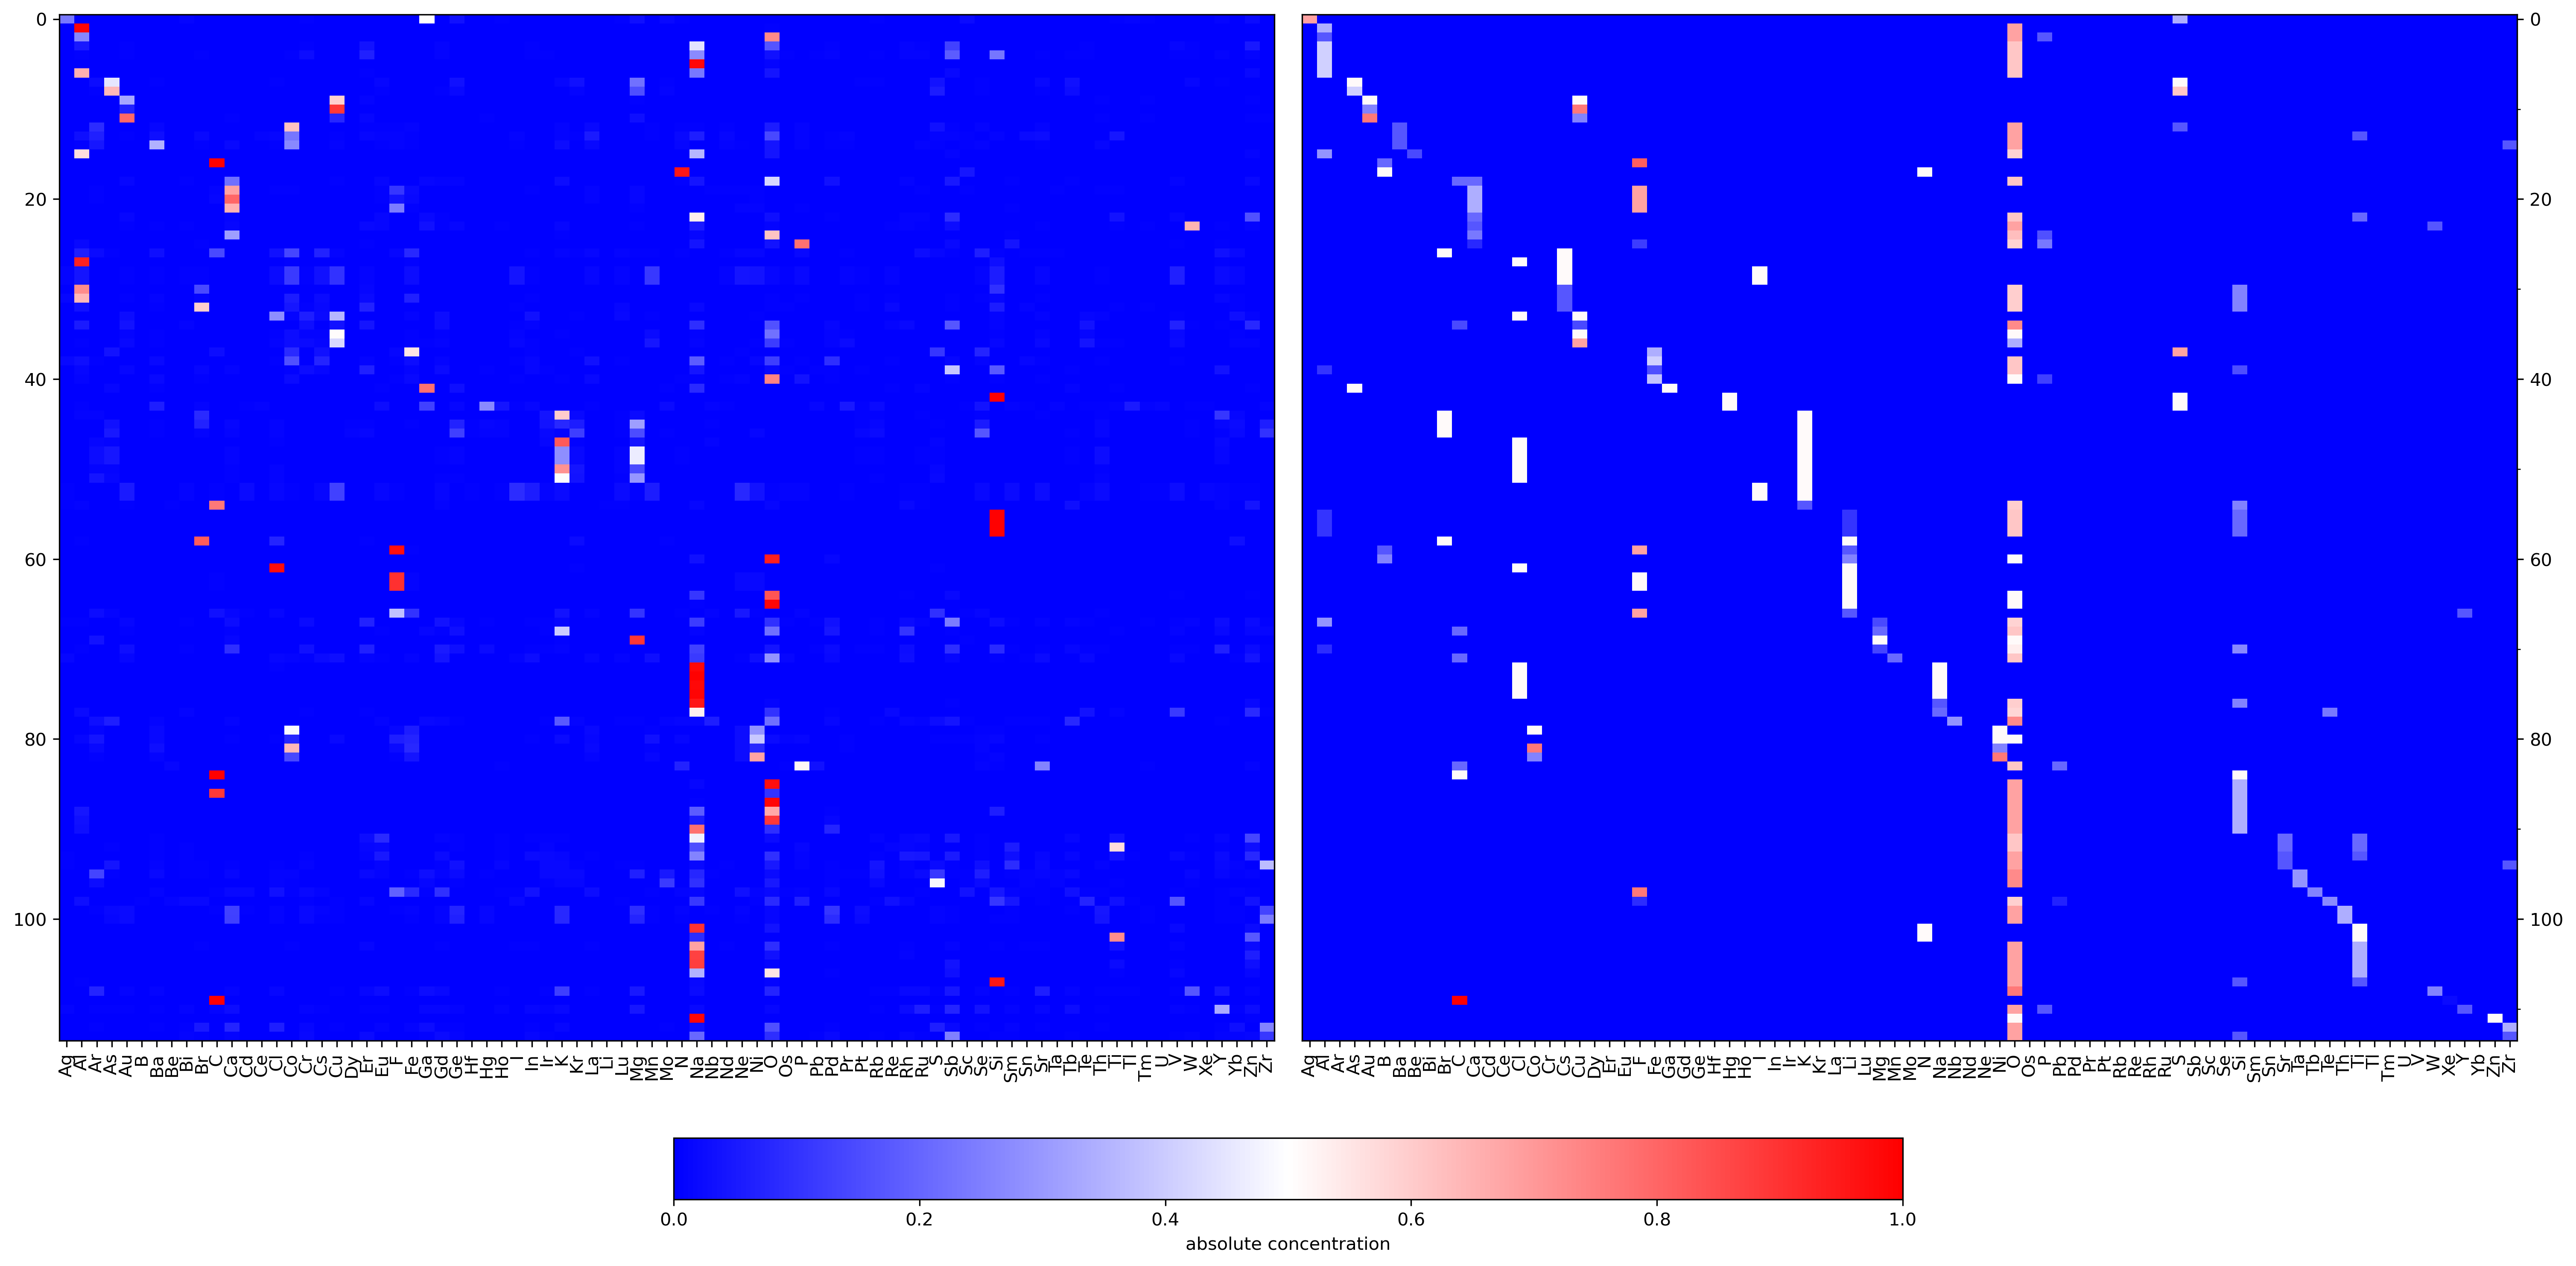
\includegraphics[width=1.2\textwidth]{Figures/cnn_dct_mae_32F_multi_best_model_pred.png}}
    \caption{The predictions of the best performing model on experimental multi-component data}
    \label{fig:multi_best_model}
\end{figure}

\begin{figure}
    \centerline{
    \centering
    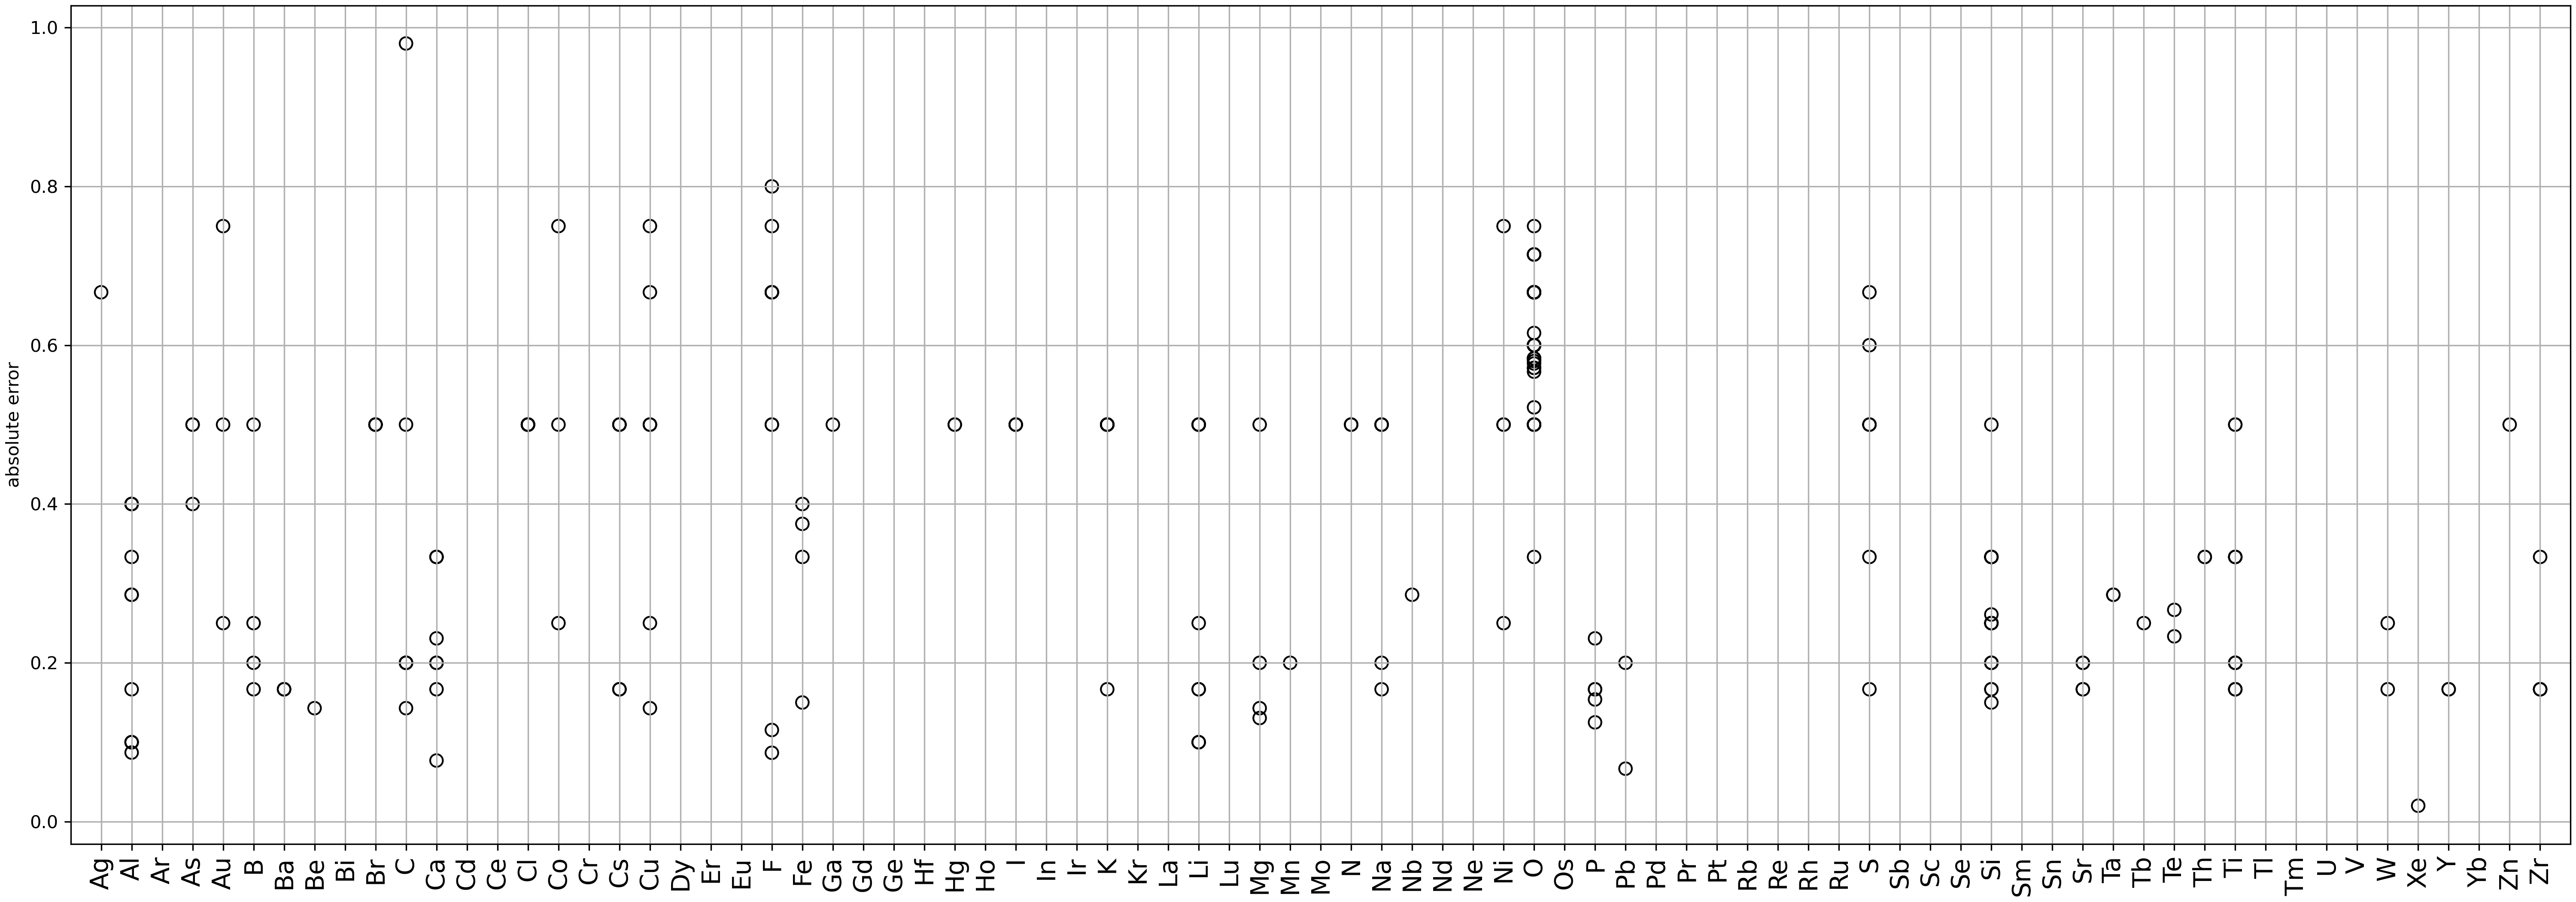
\includegraphics[width=1.1\textwidth]{Figures/mae_per_element_best_perf_multi.png}}
    \caption{The mean absolute error per element of the CNN-DCT model for quantitative prediction}
    \label{fig:boxplot}
\end{figure}

In contrast to previous studies on deep-learning assisted quantitative XPS analysis \cite{drera_deep_2019}, no relative sensitivity factors were applied in this approach. Furthermore, a significantly smaller training dataset of 30k versus the 100k which were used in their work. Lastly, the test data spectra they used were collected in experimental conditions and the training dataset was simulated according to the known conditions.

% plot visual attention feature